\documentclass[10pt]{beamer}

\usepackage{fontspec}
\usepackage{xunicode}
\usepackage{xltxtra}
\setsansfont{FreeSans}
\setmonofont{DejaVuSansMono}

\usepackage{listings}
\usepackage{textpos}
\usepackage{tikz}
\usepackage{tkz-berge}
\usepackage{minted}

\setbeamertemplate{footline}[frame]
\setbeamertemplate{items}[default]
\usetheme{Warsaw}
\usecolortheme{seahorse}
\setbeamertemplate{itemize items}[default]
\setbeamertemplate{navigation symbols}{}
\setbeamertemplate{footline}[frame number]
\setbeamertemplate{enumerate items}[default]
\lstset{columns=fixed}
\setbeamerfont*{block body}{series=\tt}
\definecolor{lightgray}{rgb}{0.9,0.9,0.9}
\definecolor{midgray}{rgb}{0.5,0.5,0.5}

\usetikzlibrary{arrows,positioning,fit,backgrounds,shapes}
\tikzset{
    %Define standard arrow tip
    >=stealth',
    thick,
    punkt/.style={
      rectangle,
      rounded corners,
      draw=black, very thick,
      text width=6.5em,
      minimum height=2em,
      text centered},
    node/.style={
      circle,
      draw=black, very thick,
      text centered},
    frogpos/.style={
      circle,
      draw=black, thick,
      text centered},
  treenode/.style = {node, ellipse}
}

\newcommand{\light}[1]{\textcolor{gray}{\footnotesize{#1}}}
\newcommand{\code}[4]{\inputminted[linenos, frame=none, firstline=#2, lastline=#3,
  framesep=10pt, bgcolor=lightgray]{#4}{#1}}

\title[aioverview]{AI с высоты птичьего полёта}
\author{Дмитрий Грошев (\href{http://twitter.com/lambdadmitry}{@lambdadmitry})}
\date{23.11.2013}

\begin{document}
\renewcommand*{\inserttotalframenumber}{\pageref{lastframe}}
\begin{frame}
\titlepage
\end{frame}

\begin{frame}{О чём пойдёт речь}
  \begin{itemize}
  \item проблема интеллекта
  \item reasoning как поиск
  \item backward-chaining
  \item forward-chaining
  \item (дискретная) оптимизация
  \item вероятности: использование и нахождение
  \end{itemize}
\end{frame}

\begin{frame}{Проблема интеллекта}
  \begin{itemize}
  \item что такое интеллект?
  \item решение задач
  \item планирование
  \item обучение
  \item самосознание?
  \end{itemize}
\end{frame}

\begin{frame}
  \Large
  Reasoning
\end{frame}

\begin{frame}{Reasoning}
  \begin{itemize}
  \item логика: все люди смертны, Сократ человек, ergo Сократ смертен
  \item алгебра: если я куплю этот Форд Фокус, придётся продать почку
  \item оптимизация: быстрее будет добраться на метро
  \item обучение: если притронуться к утюгу, будет больно
  \item вероятности: судя по выражениям лиц, меня (вероятно) будут бить
  \end{itemize}
\end{frame}

\begin{frame}[fragile]{Reasoning: Prolog}
  \begin{minted}{prolog}
mortal(X) :- human(X).
human(socrates).

?- mortal(socrates). % Yes
  \end{minted}
\end{frame}

\begin{frame}[fragile]{Завершимость}
  \begin{minted}{prolog}
arc(a, b).
arc(b, a).
arc(b, c).

path(X, Y) :- arc(X, Y).
path(X, Y) :- arc(X, Z), path(Z, Y).

?- path(a, X). % не завершится
  \end{minted}
  \begin{center}
    \begin{tikzpicture}[node distance=0.5cm]
    \node (a) [node]
          {a};
    \node (b) [node] [right=of a]
          {b}
          edge [<-,bend left]  (a)
          edge [->,bend right] (a);
    \node (c) [node] [right=of b]
          {c}
          edge [<-,bend left] (b);
    \end{tikzpicture}
  \end{center}
  \begin{center}
    miniKanren/core.logic, tabling, ASP,  …
  \end{center}
\end{frame}

\begin{frame}{Reasoning как поиск}
  \begin{itemize}
  \item reasoning как поиск в графе
  \item Prolog ищет «назад»
  \item backward-chaining
  \end{itemize}
  \begin{center}
\begin{tikzpicture}[->,>=stealth',level/.style={sibling distance = 2cm/#1,
  level distance = 1.5cm}]
\node [treenode] {path(a,X)}
  child { node[treenode]{X=a} child {node [node] {…}} }
  child { node[treenode]{X=b} child {node [node] {…}} }
  child { node[treenode]{X=c} child {node [node] {…}} };
\end{tikzpicture}
  \end{center}
\end{frame}

\begin{frame}{Поиск}
  \begin{itemize}
  \item фундаментальное понятие
  \item логика, движение в реальном мире, шамхаты, …
  \item как минимум экспоненциальный рост числа узлов в пространстве поиска
  \item эвристики: A\**, branch-and-bound, …
  \item поиск «вперёд» и «назад»
  \end{itemize}
  \begin{center}
    См. astar.gif
  \end{center}
\end{frame}

\begin{frame}{Forward-chaining}
  \begin{itemize}
  \item удивительно мало в свежей академической литературе
  \item хранилище «фактов» и, возможно, следствий
  \item вместо поиска «от цели» ищем все возможные следствия
  \item реактивные системы и «бизнес-логика»
  \item Drools, Clara
  \end{itemize}
\end{frame}

\begin{frame}[fragile]{Clara}
  \begin{minted}{clojure}
(defrule get-current-temperature
  [?current-temp <- newest-temp :from
     [TemperatureReading (== ?location location)]]
  =>
  (insert! (->CurrentTemperature
             (:value ?current-temp)
             ?location)))
  \end{minted}
\end{frame}

\begin{frame}[fragile]{Clara}
  \begin{minted}{clojure}
(defrule reduce-device-speed
  "Reduce the speed of all devices in a location
   that has a high temperature."
  [CurrentTemperature (> value high-threshold)
                      (== ?location-id location)]

  [?device <- Device (== ?location-id location)]
  =>
  (reduce-speed! ?device))
  \end{minted}
\end{frame}

\begin{frame}{Forward-chaining}
  \begin{itemize}
  \item теоретически экспоненциальная сложность
  \item на практике поддерживаются десятки тысяч правил
  \item использование в GUI?
  \item объединение с backward-chaining системами?
  \end{itemize}
\end{frame}

\begin{frame}{Constrained Logic Programming}
  \begin{itemize}
  \item уменьшение пространства поиска с помощью ограничений на значения
  \item судоку
  \end{itemize}
  \begin{center}
    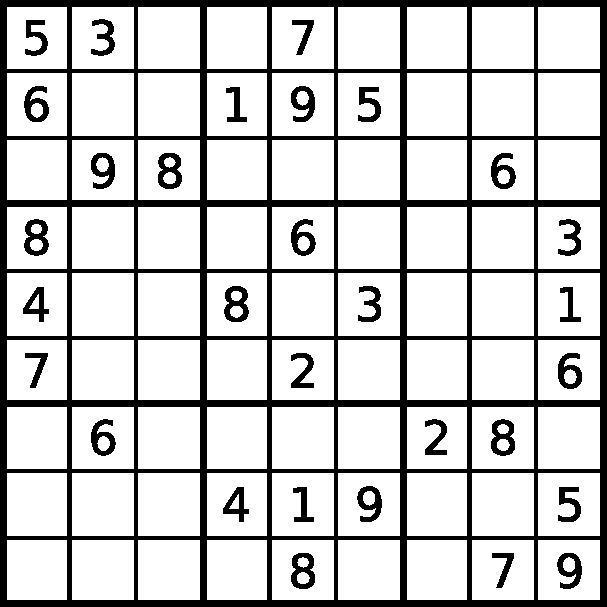
\includegraphics[height=4cm]{sudoku.pdf}
  \end{center}
\end{frame}

\begin{frame}
  \Large
  Оптимизация
\end{frame}

\begin{frame}{Возможность VS оптимальность}
  \begin{itemize}
  \item «возможное» (feasible) $\neq$ «оптимальное»
  \item целевая функция: оптимизируемое значение
  \item оптимизация: перебор возможных вариантов
  \item возможность: оптимизация без целевой функции
  \end{itemize}
\end{frame}

\begin{frame}{Задача о рюкзаке}
  \begin{itemize}
  \item целевая функция: максимальная стоимость
  \item ограничение: вместимость рюкзака
  \end{itemize}
  \begin{center}
    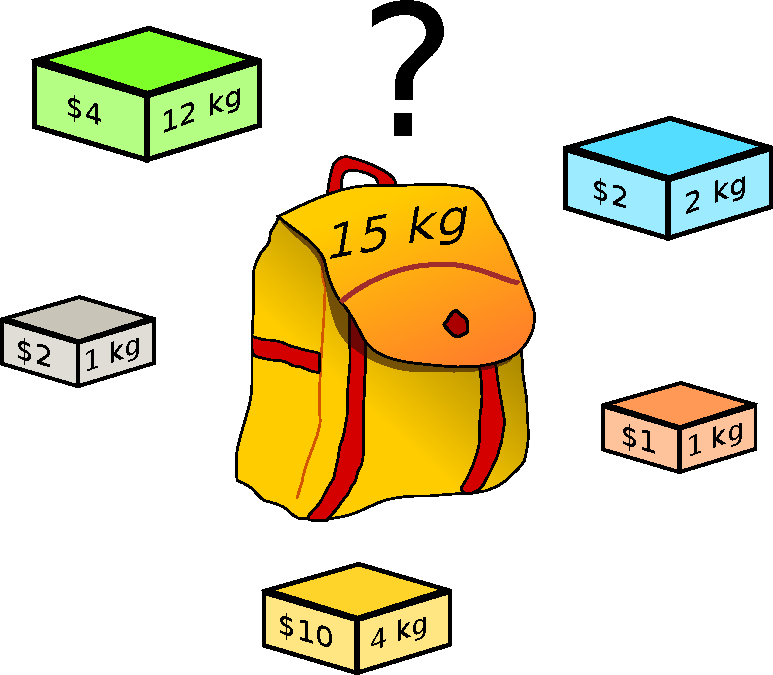
\includegraphics[height=4cm]{knapsack.pdf}
  \end{center}
\end{frame}

\begin{frame}{Задача о коммивояжёре}
  \begin{itemize}
  \item целевая функция: минимальная стоимость
  \item ограничение: однократное посещение всех вершин, кроме одной
  \end{itemize}
  \begin{center}
  \begin{tikzpicture}[scale=0.75]
    % \GraphInit[]
    \SetVertexMath
    \grEmptyCycle[RA=3, rotation=90]{5}

    \tikzset{EdgeStyle/.append style = {bend left}}
    \Edge[label=$7$](a0)(a4)
    \Edge[label=$2$,lw=2pt](a0)(a3)
    \Edge[label=$3$,lw=2pt](a1)(a4)

    \tikzset{EdgeStyle/.append style = {bend right}}
    \Edge[label=$8$](a2)(a4)
    \Edge[label=$4$,lw=2pt](a0)(a2)
    \Edge[label=$6$](a1)(a3)

    \Edge[label=$5$](a2)(a3)
    \Edge[label=$6$,lw=2pt](a3)(a4)
    \Edge[label=$3$](a0)(a1)
    \Edge[label=$4$,lw=2pt](a1)(a2)
  \end{tikzpicture}
  \end{center}
\end{frame}

\begin{frame}{Глобальная оптимизация}
  \begin{itemize}
  \item линейная (Симплекс-алгоритм)
  \item дискретная (MIP, C(L)P, SAT)
  \item нелинейная (?)
  \end{itemize}
\end{frame}

\begin{frame}{Локальная оптимизация}
  \begin{itemize}
  \item hill climbing и жадные алгоритмы
  \item локальные оптимумы и пертурбации
  \item simulated annealing, генетические алгоритмы, …
  \end{itemize}
\end{frame}

\begin{frame}{Планирование}
  \begin{itemize}
  \item обычно есть целевая функция
  \item обычно много нетривиальных ограничений
  \item непосредственно применимо на практике
  \end{itemize}
\end{frame}

\begin{frame}
  \Large
  Вероятности и Machine Learning
\end{frame}

\begin{frame}{Вероятности}
  \begin{itemize}
  \item неуверенность в окружающем мире
  \item мера понимания мира: вероятность
  \item ML
  \item использование вероятностей
  \item нахождение вероятностей (обучение)
  \end{itemize}
\end{frame}

\begin{frame}{Использование вероятностей}
  \begin{itemize}
  \item maximum likelihood
  \item недоверенные датчики: markov chain
  \item вероятностная state machine: markov decision process (MDP)
  \item и то, и другое: partially observable markov decision process (POMDP)
  \end{itemize}
\end{frame}

\begin{frame}{Нахождение вероятностей/обучение}
  \begin{itemize}
  \item supervised learning (вывод функции)
  \item классификация (на этой картинке изображён котик!)
  \item регрессия и предсказание (цена дома через год)
  \item unsupervised learning (анализ данных)
  \item кластеризация
  \end{itemize}
  \begin{center}
    Нейронные сети — всего лишь классификатор
  \end{center}
\end{frame}

\begin{frame}
  \Large
  Примеры
\end{frame}

\begin{frame}{Поисковые системы}
  \begin{itemize}
  \item гигантские классификаторы
  \item проблема ­ масштаб, а не концептуальная сложность
  \end{itemize}
\end{frame}

\begin{frame}{Автоматизированный перевод}
  \begin{itemize}
  \item старый подход: reasoning о структуре фразы
  \item новый подход: статистический перевод (классификация)
  \end{itemize}
\end{frame}

\begin{frame}{Google self-driving car}
  \begin{itemize}
  \item (дискретная) оптимизация для нахождения пути
  \item планирование пути
  \item вероятностная локализация
  \item классификация препятствий
  \end{itemize}
\end{frame}

\begin{frame}
  \Large
  Заключение
\end{frame}

\begin{frame}{В шляпе кончились кролики}
  \begin{itemize}
  \item в «разумном» поведении нет магии, только трюки
  \item самосознание можно имитировать
  \item что такое интеллект?
  \end{itemize}
  \begin{center}
    Слайды: \url{https://github.com/si14/sprug-2013-11-slides}
  \end{center}
\end{frame}

\begin{frame}{Использованные материалы}\label{lastframe}
  \footnotesize
  \begin{itemize}
  \item \url{http://en.wikipedia.org/wiki/File:Knapsack.svg}
  \end{itemize}
\end{frame}
